\documentclass[10pt]{article}
\usepackage[margin=0.62in]{geometry}
\usepackage{times}
\usepackage{amsmath,amssymb}
\usepackage{booktabs,tabularx,array}
\usepackage{float}
\usepackage{enumitem}
\usepackage{microtype}
\usepackage{hyperref}
\usepackage{xcolor}
\usepackage{tikz}
\usetikzlibrary{arrows.meta,positioning,fit,calc,shapes.geometric}
\hypersetup{hidelinks}

\floatstyle{ruled}
\newfloat{algorithm}{htbp}{loa}
\floatname{algorithm}{Algorithm}

\definecolor{primitivecol}{RGB}{85,85,85}
\definecolor{optioncol}{RGB}{183,83,42}
\definecolor{landmarkcol}{RGB}{42,104,155}
\definecolor{observedcol}{RGB}{225,225,225}
\newcolumntype{Y}{>{\raggedright\arraybackslash}X}
\newcolumntype{P}[1]{>{\raggedright\arraybackslash}p{#1}}
\setlength{\parindent}{0pt}
\setlength{\parskip}{2.5pt}
\setlength{\textfloatsep}{7pt}
\setlist{nosep,leftmargin=5mm}
\renewcommand{\arraystretch}{1.12}

\tikzset{
  obsv/.style={circle,draw,fill=observedcol,minimum size=8mm,inner sep=1pt,font=\small},
  hid/.style={circle,draw=landmarkcol,fill=landmarkcol!18,line width=1pt,minimum size=8mm,inner sep=1pt,font=\small},
  ntm/.style={rectangle,rounded corners=2pt,draw=optioncol,fill=optioncol!18,line width=1pt,inner sep=2.5pt,font=\small},
  arr/.style={-{Stealth[length=3pt]},line width=0.7pt}
}

\begin{document}

\begin{center}
{\LARGE\bfseries Inference and Structure Learning by Bayesian Structural EM}\\[2pt]
{\large Analysis 8: recovering the agent's static representation from behavior}\\[3pt]
{\small 7 June 2026}
\end{center}

\begin{abstract}
Analysis 7 fixed the \emph{generative} model: a static, task-independent representation
$\mathcal R_M$ induces a cognitive map, a search kernel selects latent assignments $z$, and an
execution model emits behavior. This note treats the \emph{inverse} problem: given
trajectories, recover the family $M$, the representation $\mathcal R_M$, the continuous
parameters $\Theta_M$, and whatever latent assignment remains. The umbrella algorithm is
Friedman's \emph{Bayesian Structural EM}. Its two families read differently inside this
umbrella: the action-chunk family is \emph{grammar induction with a per-occurrence parse}
$z^{g}$, whereas the landmark family is \emph{graph clustering} --- learning the static
membership $z^{\ell}:\mathcal S\to\mathcal L$ and the region graph $\mathcal E^{\mathcal L}$,
a hidden mediating layer over observed states in the sense of Friedman's hidden-variable
networks (his Fig.~1b).
\end{abstract}

\section{The inverse problem}

Given $\mathcal D=\{\tau_n\}_{n=1}^N$, infer
\begin{equation}
p(M,\mathcal R_M,\Theta_M,z\mid\mathcal D).
\label{eq:inverse}
\end{equation}
$M$ selects a family; $\mathcal R_M$ is the static stored knowledge; $\Theta_M$ governs
search and execution; $z$ is the latent assignment lifting primitives to the abstract layer.
The exact evidence $p(M\mid\mathcal D)\propto p(M)\sum_{\mathcal R_M}\int\sum_z
p(\mathcal D,z,\mathcal R_M,\Theta_M\mid M)\,d\Theta_M$ is intractable, which is the setting
Structural EM was built for.

\section{What is hidden, and the two modes}

Recall from Analysis 7 that the segmentation $\chi$ is \emph{derived}: once $z$ is fixed, the
runs of constant assignment fix the boundaries. The genuine hidden object is $z$, and it
sits differently in the two families (Figure~\ref{fig:hidden}).

\emph{Action chunk (a parse).} The static knowledge is the grammar $\mathcal G$ over actions;
applying it to a trajectory requires a \emph{per-occurrence} parse $z^{g}_{n,t}$ (which
production generated each action). Inference is grammar induction with a hidden parse ---
HSMM/PCFG-style.

\emph{Landmark (a clustering).} The static knowledge is the membership $z^{\ell}:\mathcal
S\to\mathcal L$ together with the region graph $\mathcal E^{\mathcal L}$. Because membership is
static and states are observed, the per-trajectory region sequence
$z^{\ell}(s_{n,t})$ is \emph{determined}; there is no per-trajectory parse latent. The hidden
object is the partition itself --- a hidden node that mediates a group of observed states
(Friedman, Fig.~1b). Inference is therefore \emph{graph clustering / stochastic-block-model}
structure learning: which states share a region, and how regions connect.

\begin{figure}[H]
\centering
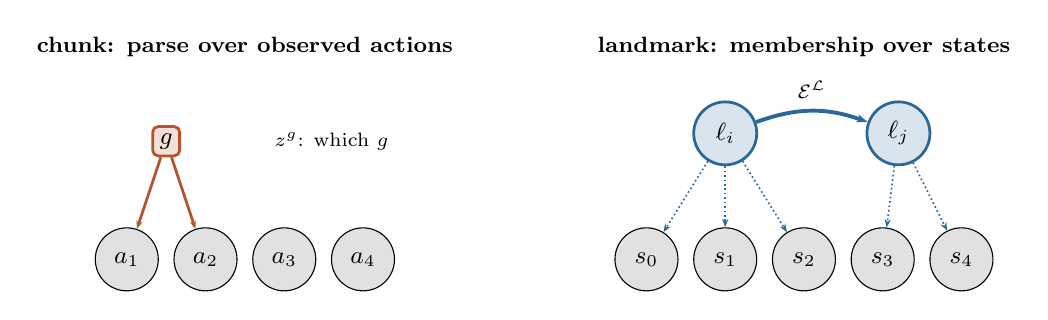
\begin{tikzpicture}[x=1cm,y=1cm]
  \node[font=\bfseries\footnotesize] at (1.5,2.7) {chunk: parse over observed actions};
  \node[obsv] (a1) at (0,0) {$a_1$};\node[obsv] (a2) at (1,0) {$a_2$};
  \node[obsv] (a3) at (2,0) {$a_3$};\node[obsv] (a4) at (3,0) {$a_4$};
  \node[ntm] (g) at (0.5,1.5) {$g$};
  \draw[-{Stealth[length=3pt]},optioncol,line width=1pt] (g)--(a1);
  \draw[-{Stealth[length=3pt]},optioncol,line width=1pt] (g)--(a2);
  \node[font=\scriptsize] at (2.6,1.5) {$z^{g}$: which $g$};
  \begin{scope}[xshift=6.6cm]
  \node[font=\bfseries\footnotesize] at (2,2.7) {landmark: membership over states};
  \node[obsv] (s0) at (0,0) {$s_0$};\node[obsv] (s1) at (1,0) {$s_1$};
  \node[obsv] (s2) at (2,0) {$s_2$};\node[obsv] (s3) at (3,0) {$s_3$};\node[obsv] (s4) at (4,0) {$s_4$};
  \node[hid] (li) at (1,1.6) {$\ell_i$};\node[hid] (lj) at (3.2,1.6) {$\ell_j$};
  \draw[-{Stealth[length=3pt]},landmarkcol,line width=0.6pt,densely dotted] (li)--(s0);
  \draw[-{Stealth[length=3pt]},landmarkcol,line width=0.6pt,densely dotted] (li)--(s1);
  \draw[-{Stealth[length=3pt]},landmarkcol,line width=0.6pt,densely dotted] (li)--(s2);
  \draw[-{Stealth[length=3pt]},landmarkcol,line width=0.6pt,densely dotted] (lj)--(s3);
  \draw[-{Stealth[length=3pt]},landmarkcol,line width=0.6pt,densely dotted] (lj)--(s4);
  \draw[-{Stealth[length=4pt]},landmarkcol,line width=1.4pt] (li) to[bend left=20] (lj);
  \node[font=\scriptsize] at (2.1,2.15) {$\mathcal E^{\mathcal L}$};
  \end{scope}
\end{tikzpicture}
\caption{The two modes of hidden structure. \emph{Left}: a chunk $g$ generates a span of
observed actions; the hidden parse $z^{g}$ says which production. \emph{Right}: a landmark
$\ell$ owns a group of observed states through the static membership $z^{\ell}$ (dotted),
with region links $\mathcal E^{\mathcal L}$ (solid) --- a hidden mediating layer, à la
Friedman's Fig.~1b. Chunk inference is parsing; landmark inference is clustering.}
\label{fig:hidden}
\end{figure}

\section{Bayesian Structural EM}

Structural EM \cite{friedman1998} searches the joint space of (structure $\times$ parameters):
each step either improves $\Theta_M$ for the current structure, or proposes a new structure
scored \emph{not} by re-running full inference but by the expected sufficient statistics of
the current completion. The loop is
$z\leftrightarrow\Theta_M\leftrightarrow\mathcal R_M$, regenerating
$\mathcal K_M=F_M(\mathcal K_0,\mathcal R_M)$ after every representation update. We keep the
Bayesian (BDeu) marginal likelihood as a within-family \emph{proposal diagnostic} and accept
moves on a unified observed-data score so that families with different vocabularies stay
comparable.

\section{E-step}

\subsection{Chunk mode: weighted parsing}

Build a span lattice $\Lambda_n(\mathcal G)$ on boundaries $\{0,\ldots,T_n\}$. Primitive arcs
$(t-1)\xrightarrow{a_{n,t}}t$ are always present; a chunk arc $(u-1)\xrightarrow{g}v$ exists
iff $a_{n,u:v}=g$ is executable from $s_{n,u-1}$. With arc weight
\begin{equation}
w_{n,u,v,z}^{(r)}
=p_{\mathrm S}(z\mid s_{n,u-1},s_{\star,n},\mathcal K_M,\theta_{\mathrm S}^{(r)})\,
p_{\mathrm E}(\tau_{n,u:v}\mid z,\theta_{\mathrm E}^{(r)},\mathcal K_0),
\label{eq:arcw}
\end{equation}
forward--backward gives parse responsibilities
$\gamma_{n,u,v,z}^{(r)}=\operatorname{Fwd}_n(u-1)\,w^{(r)}_{n,u,v,z}\,\operatorname{Bwd}_n(v)/\operatorname{Fwd}_n(T_n)$.

\subsection{Landmark mode: membership posterior}

Here the latent is the static partition. For region graph $\mathcal E^{\mathcal L}$ and
parameters $\Theta_M^{(r)}$, the E-step is the posterior over each state's membership,
\begin{equation}
r_s^{(r)}(\ell)
=p\!\left(z^{\ell}(s)=\ell \,\middle|\, \mathcal D,\mathcal E^{\mathcal L},\Theta_M^{(r)}\right)
\ \propto\
\underbrace{p(z^{\ell}(s)=\ell)}_{\text{Voronoi prior, A7 Eq.~(4)}}\
\prod_{n,t:\,s_{n,t}=s}\!\!
p\bigl(\text{out-transition of }s_{n,t}\mid z^{\ell}(\cdot),\mathcal E^{\mathcal L},\Theta_M^{(r)}\bigr).
\label{eq:membership}
\end{equation}
States that enter and leave the same regions in the same way are pulled into the same block;
this is the stochastic-block-model coupling. No per-trajectory parse is summed over --- given
a membership, region labels and crossings $\chi^{\ell}$ are read off the observed path.

\section{M-step}

Holding $\mathcal R_M$ fixed,
\begin{equation}
\Theta_M^{(r+1)}
=\arg\max_{\Theta_M}\sum_n\mathbb E^{(r)}\!\left[\log p(\tau_n,z_n\mid M,\mathcal R_M,\Theta_M)\right]
-\mathcal P_M(\Theta_M),
\label{eq:mstep}
\end{equation}
where the expectation is over parse responsibilities (chunk) or membership responsibilities
(landmark). Expected counts update the search sensitivity $\beta\in\theta_{\mathrm S}$ and the
execution sharpness $\eta\in\theta_{\mathrm E}$.

\section{Structure step}

A proposal $\mathcal R_M\to\mathcal R'_M$ regenerates $\mathcal K'_M$ and must be re-scored.
Candidate-compatible expected counts $\bar N_M^{(r)}(\mathcal R'_M)$ are formed from the
re-evaluated responsibilities, ranked by the BDeu diagnostic
\begin{equation}
\mathcal B_M^{(r)}(\mathcal R'_M)
=\log p_{\mathrm{BDeu}}\!\bigl(\bar N_M^{(r)}(\mathcal R'_M)\mid\mathcal R'_M,\alpha_{\mathrm{BD}}\bigr)
+\log p(\mathcal R'_M\mid M),
\label{eq:bdeu}
\end{equation}
and accepted only on the unified observed-data score
\begin{equation}
\mathcal C_M(\mathcal R'_M)
=\sum_n\log p(\tau_n\mid M,\mathcal R'_M,\widehat\Theta_M(\mathcal R'_M))
+\log p(\mathcal R'_M\mid M).
\label{eq:accept}
\end{equation}
Family-specific moves:
\begin{itemize}
\item \textbf{Chunk:} add / remove / split / merge productions in $\mathcal G$ (recursive
non-terminals allowed). Each changes the parse lattice.
\item \textbf{Landmark:} add / remove / relocate a landmark; \emph{re-assign} states between
regions (membership moves); add / remove a region edge in $\mathcal E^{\mathcal L}$. These are
clustering moves on the state graph plus edits to the region graph.
\end{itemize}

\section{The algorithm}

Algorithm~\ref{alg:bsem} is the synchronized loop with its two modes. It is analyst-side
inference and makes no claim that participants run EM.

\begin{algorithm}[H]
\caption{Bayesian Structural EM for agent structure learning}
\label{alg:bsem}
\small
\begin{flushleft}
\textbf{Input:} trajectories $\mathcal D=\{\tau_n\}$, family $M$, base map $\mathcal K_0$,
priors $p(\mathcal R_M\mid M),\,p(\Theta_M\mid M)$\\
\textbf{Output:} $\widehat{\mathcal R}_M,\widehat\Theta_M$, responsibilities\\[3pt]
\textbf{1.}\ \ initialize $\mathcal R_M$ ($\mathcal G=\varnothing$, or seed $z^{\ell}$ by Voronoi from $d^{*}$) and $\Theta_M$; build $\mathcal K_M$\\
\textbf{2.}\ \ \textbf{repeat}\\
\hspace*{1.4em}\textbf{3. E-step (mode by family):}\\
\hspace*{3.0em}\emph{chunk} --- parse every $\Lambda_n(\mathcal G)$ [Eq.~\eqref{eq:arcw}]; forward--backward $\Rightarrow$ parse resp.\ $\gamma$\\
\hspace*{3.0em}\emph{landmark} --- membership posterior $r_s(\ell)$ over states [Eq.~\eqref{eq:membership}] (clustering)\\
\hspace*{1.4em}\textbf{4. M-step:} $\Theta_M\gets\arg\max\ \mathbb E[\log p(\tau,z\mid\cdot)]-\mathcal P_M$ [Eq.~\eqref{eq:mstep}]\\
\hspace*{1.4em}\textbf{5. Structure step:} generate moves\\
\hspace*{3.0em}\emph{chunk}: add/remove/split/merge productions in $\mathcal G$\\
\hspace*{3.0em}\emph{landmark}: add/remove/relocate landmark, re-assign membership, edit $\mathcal E^{\mathcal L}$\\
\hspace*{1.4em}\textbf{6.}\ \ for each move $\mathcal R'_M$: regenerate $\mathcal K'_M$, re-evaluate responsibilities, counts $\bar N(\mathcal R'_M)$; rank by BDeu $\mathcal B_M$ [Eq.~\eqref{eq:bdeu}]\\
\hspace*{1.4em}\textbf{7.}\ \ for top-ranked: refit $\widehat\Theta_M(\mathcal R'_M)$; accept the move maximizing $\mathcal C_M$ \textbf{if} it improves [Eq.~\eqref{eq:accept}]\\
\textbf{8.}\ \ \textbf{until} $\mathcal C_M$ stabilizes;\quad\textbf{return} $\mathcal R_M,\Theta_M$, responsibilities
\end{flushleft}
\end{algorithm}

The primitive family has no structure step. Both discrete searches are nonconvex; the
landmark (hidden-membership) case has more pronounced local optima, so random restarts and
membership perturbations are advisable --- exactly the difficulty Friedman notes for
hidden-variable structure learning.

\section{Model comparison}

For each family, $\widehat\ell_M=\sum_n\log p(\tau_n\mid M,\widehat{\mathcal R}_M,\widehat\Theta_M)$.
The primary cross-family comparison is held-out predictive likelihood, which scores the same
observed data for every family. A secondary BIC/Laplace summary uses
$\mathrm{IC}_M=-2\widehat\ell_M+k_M\log N_{\mathrm{eff}}-2\log p(\widehat{\mathcal R}_M\mid M)$,
$N_{\mathrm{eff}}=\sum_n T_n$, with approximate probabilities
$\widetilde p(M\mid\mathcal D)\propto p(M)\exp(-\tfrac12\mathrm{IC}_M)$. Raw BDeu diagnostics
are not compared across families, whose token spaces differ.

\section{What identifies the families, and recovery}

\begin{table}[H]
\centering
\small
\begin{tabularx}{\textwidth}{lY}
\toprule
Observed pattern & Main evidential implication \\
\midrule
Same action string recurs across locations & a reusable production in $\mathcal G$. \\
States with interchangeable in/out transitions & a shared region in $z^{\ell}$ (a block). \\
Different routes converge on the same region boundary & a region edge in $\mathcal E^{\mathcal L}$. \\
Routes / RT predicted by shortcut-induced fewer expansions & the map-mediated search account. \\
Boundaries without stable strings or stable regions & insufficient: both families fit generic segmentation. \\
\bottomrule
\end{tabularx}
\caption{Identifying observations. Signatures are necessary but not sufficient.}
\label{tab:identification}
\end{table}

\textbf{Recovery protocol.} Simulate known families and representations; fit all candidates
with Algorithm~\ref{alg:bsem} for $\alpha_{\mathrm{BD}}\in\{0.1,1,5,10\}$; verify the
generating family and (for landmark) the generating \emph{partition} are recovered; only then
interpret human assignments. The key landmark question is whether a learned clustering of
states into regions, plus a region graph, predicts held-out behavior better than the
primitive baseline while primitive transitions remain available.

\section{Take-home}

The agent families live in the generative model of Analysis 7; this note recovers them.
Bayesian Structural EM is one umbrella with two modes: ``add a production'' is a move in
\emph{grammar induction over actions} with a hidden parse, while ``re-assign a state'' or
``add a region edge'' is a move in \emph{graph clustering over states} with a hidden static
membership (Fig.~\ref{fig:hidden}) --- the same algorithm, differing only in whether the
hidden structure is a parse or a partition.

\begin{thebibliography}{9}
\bibitem{friedman1998} N.\ Friedman. The Bayesian Structural EM Algorithm.
\emph{Proc.\ 14th Conf.\ on Uncertainty in Artificial Intelligence (UAI)}, 1998. arXiv:1301.7373.
\end{thebibliography}

\end{document}
